\documentclass[10pt,twocolumn]{article}
\usepackage[utf8]{inputenc}
\usepackage[spanish]{babel}
\usepackage{amsmath, amssymb, amsthm}
\usepackage{graphicx, subfigure, epsfig}
\usepackage{geometry}
\usepackage{color, xcolor}
\usepackage{hyperref}
\usepackage{parskip}
\usepackage{tikz}
\usetikzlibrary{shapes,arrows}
\tikzstyle{block} = [rectangle, draw, text width=7.5em, text centered, rounded corners, node distance=4cm, minimum height=4em]
\tikzstyle{line} = [draw, -latex']
\usepackage{appendix}
\usepackage{caption}

\hypersetup{
	colorlinks,
	linkcolor={red!50!black},
	citecolor={blue!50!black},
	urlcolor={blue!80!black}
}

\newtheorem{eg}{Example}[section]

\begin{document}
	\title{Planeador de Excursiones}
	\author{
		Amanda Cordero Lezcano\\
		Christopher Guerra Herrero\\
		Alfredo Nuño Oquendo\\Facultad de Matemática y Computación, Universidad de La Habana
	}
	\date{Septiembre, 2024}
	
	\twocolumn[
	\begin{@twocolumnfalse}
		\maketitle
		\begin{abstract}
			Esta investigación presenta una simulación de un grupo de personas en una excursión, donde se recolectan características de los excursionistas mediante encuestas. Posteriormente, utilizando la metaheur\'istica Recocido simulado y varias simulaciones para computar el costo de las rutas, se planifica una ruta con elevado nivel de satisfacción de los participantes. De esta, se elabora un pequeño anuncio por medio de un modelo de lenguaje. Finalmente, se simula la excursión con un modelo basado en agentes BDI y un controlador difuso para ajustar los tiempos de espera de los excursionistas en diferentes puntos del recorrido.
		\end{abstract}
		\vspace{1cm}
	\end{@twocolumnfalse}
	]
	\section{Introducción}
	El objetivo de esta investigación es simular una excursión con un grupo de excursionistas basándose en sus preferencias individuales, las características del terreno y las rutas disponibles. Para ello, se recolecta información de los excursionistas a través de encuestas. Se utiliza la metaheur\'istica Recocido simulado y varias simulaciones para computar el costo de las rutas y tomar la mejor en cuanto a la satisfacción de los participantes. Se elabora un anuncio usando el modelo de lenguaje Mistral Large 2. Se simula mediante agentes BDI, usando un controlador difuso para computar el tiempo de espera de los campistas.
	
	\subsection{Objetivos}
	Los principales objetivos de esta investigación son:
	\begin{itemize}
		\item Planificar rutas óptimas que maximicen la satisfacción de los excursionistas.
		\item Elaborar un anuncio llamativo para los excursionistas.
		\item Detectar puntos críticos en el recorrido que puedan mejorar la experiencia en excursiones reales.
		\item Crear una plataforma amigable para el guía de la excursión.
	\end{itemize}
	
	\section{Fundamento Matemático}
	Los fundamentos matemáticos de las técnicas utilizadas para implementar la simulación: metaheur\'istica Recocido simulado, el modelo de agentes BDI y el controlador difuso.
	
	\subsection{Recocido simulado}
	
	El recocido simulado (simulated annealing) es una técnica de optimización inspirada en el proceso de recocido en metalurgia. Su objetivo es encontrar una solución aproximada a problemas complejos.
	Utiliza una búsqueda aleatoria que permite explorar soluciones vecinas, aceptando no solo mejoras, sino también soluciones peores con cierta probabilidad. Esto ayuda a evitar quedar atrapado en óptimos locales.
	La temperatura es un parámetro que controla la aceptación de soluciones peores. Al inicio, la temperatura es alta, lo que permite explorar ampliamente el espacio de soluciones. A medida que avanza el proceso, la temperatura disminuye, restringiendo la búsqueda y favoreciendo la convergencia hacia una solución óptima.
	
	
	\subsection{Modelo de Agentes BDI}
	El modelo BDI (Belief-Desire-Intention) se basa en la lógica modal para representar el comportamiento racional de los agentes. Los agentes tienen:
	\begin{itemize}
		\item Creencias (\(B\)): Representan lo que el agente sabe o cree acerca del mundo.
		\item Deseos (\(D\)): Los objetivos que el agente intenta alcanzar.
		\item Intenciones (\(I\)): Los planes o acciones que el agente ha decidido ejecutar para lograr sus deseos.
	\end{itemize}
	
	Matemáticamente, el comportamiento de los agentes se puede describir usando una estructura modal \( \langle B, D, I \rangle \), donde cada componente se actualiza según las reglas del sistema. La lógica BDI sigue el principio de que las intenciones deben ser consistentes con las creencias y deseos actuales.
	
	\subsection{Controlador Difuso}
	
	En general, los controladores difusos son sistemas expertos especiales. Cada uno emplea una base de conocimientos, expresada en términos de reglas de inferencia difusa relevantes, y un motor de inferencia adecuado para resolver un problema de control determinado. Los controladores difusos varían sustancialmente según la naturaleza de los problemas de control que se supone deben resolver. Los problemas de control van desde tareas complejas, típicas en robótica, que requieren una multitud de acciones coordinadas, hasta objetivos simples, como mantener un estado prescrito de una sola variable.\cite{Fuzzy}
	
	Un controlador difuso general consiste en cuatro módulos: una base de reglas difusas, un motor de inferencia difusa, y módulos de fuzzificación/defuzzificación. Las interconexiones entre estos módulos y el proceso controlado se muestran en la Figura \ref{fig:diagram}.
	
	\begin{figure*}[h]
		\centering
		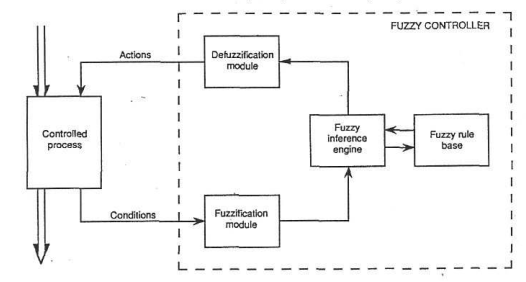
\includegraphics[width=\linewidth]{diagram}
		\caption{Imagen extraída de \cite{Fuzzy}. Esquema general de un controlador difuso}
		\label{fig:diagram}
	\end{figure*}
	
	
	\section{Detalles de Implementación}
	
	Se desarrolló un sitio web en Django para interactuar con el guía de la excursión. En el mismo se encuentra una encuesta para los excursionistas, con la cual se obtendrán datos sobre sus preferencias. Posteriormente, el guía puede introducir en la plataforma el mapa de la región de interés.
	
	 El costo de la simulaci\'on est\'a dado por el opuesto del beneficio. El beneficio de una simulacii\'on comienza en cero. Cada excursionitsta en cada punto aporta al beneficio el resultado de calcular el producto escalar entre sus preferencias y las caracter\'isticas del sitio. Adem\'as el beneficio se ve afectado tambi\'en de forma fija por los puntos de reagrupaci\'on, almuerzo y campamento. 
	 
	 Usamos Recocido simulado para obtener una buena ruta. Se selecciona una ruta inicial mediante un algoritmo para hallar caminos de costo m\'inimo(Dijkstra), se eval\'ua esta hallando el costo de una simulaci\'on de la misma. Luego si la temperatura no ha rebasado un umbral, se modifica la ruta acorde a lo planteado por la metaheur\'istica. Este proceso contin\'ua hasta que el metal se haya enfriado o el costo de las simulaciones se haya estabilizado(la desviaci\'on est\'andar de los costos entre, la ra\'iz de la cantidad de observaciones por la media de las observaciones, haya alcanzado un umbral). En la figura \ref{fig:diagram} se muestra un mapa sobre el que ocurri\'o este proceso. Una arista es m\'as oscura si m\'as caminos pasaron por esta en el proceso.
	 
		 \begin{figure*}[h]
		 	\centering
		 	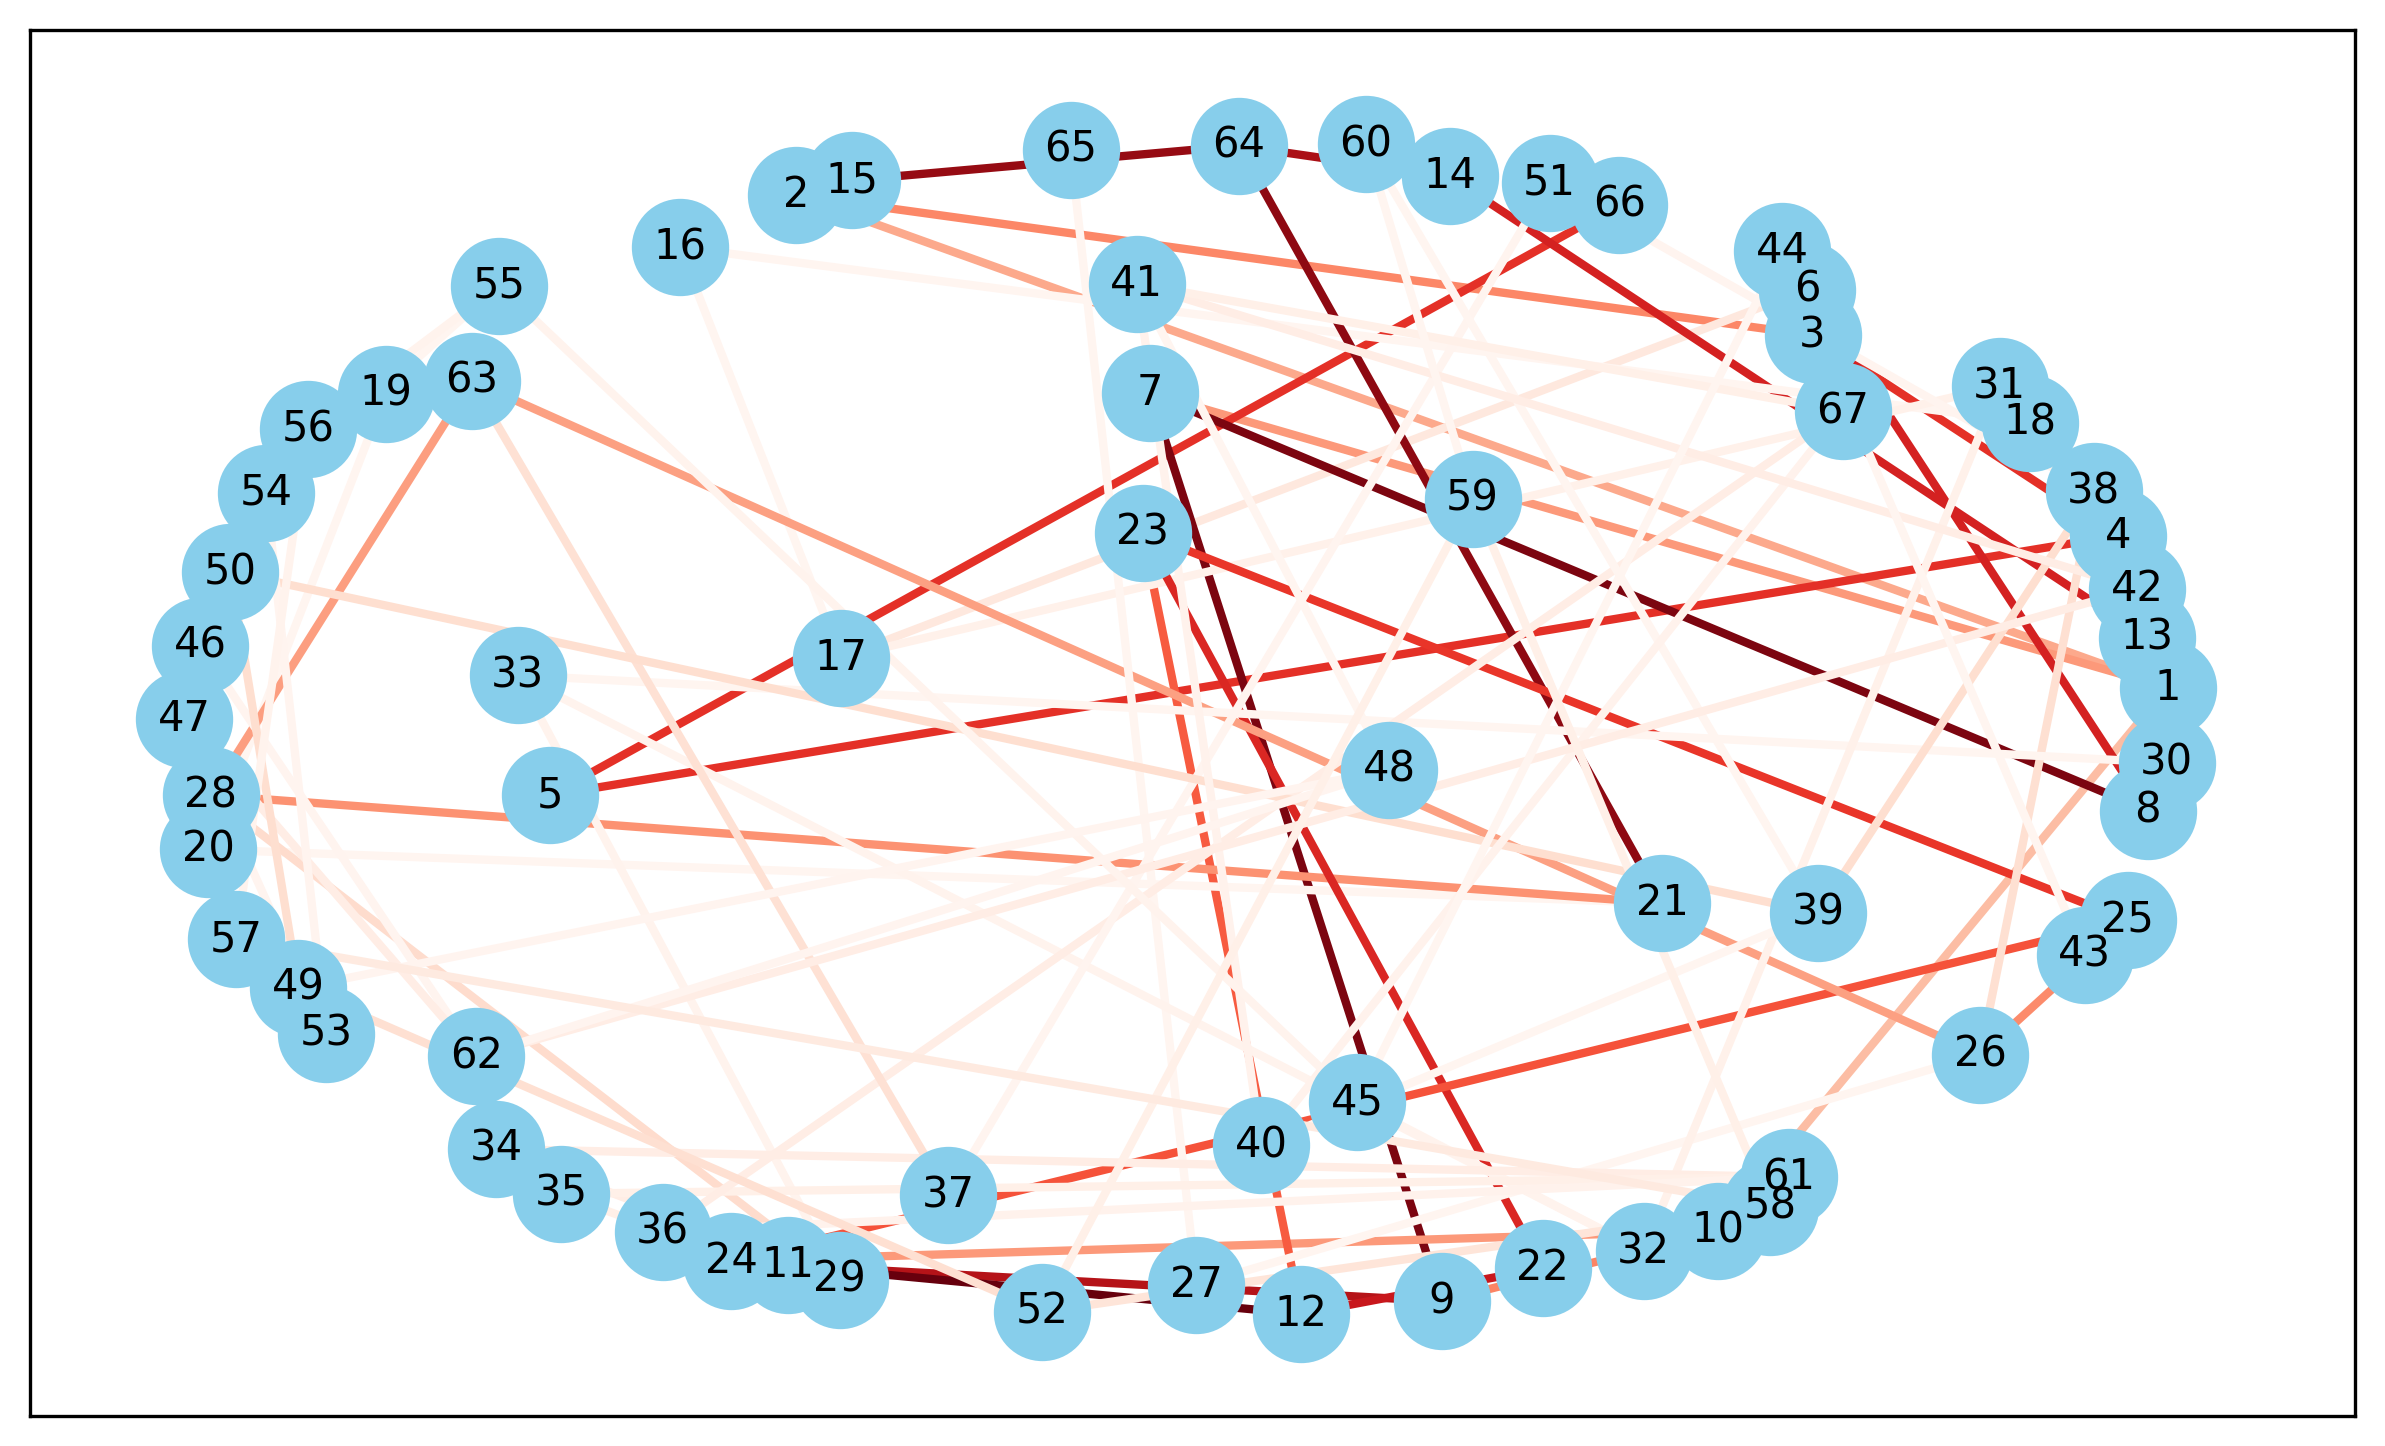
\includegraphics[width=\linewidth]{routes_stats.png}
		 	\caption{}
		 	\label{fig:routesstats}
		 \end{figure*}
	
	 

	 
	 Luego se muestra en la web un anuncio elaborado por el modelo de lenguaje Mistral Large 2, a partir de las características del camino seleccionado.\\
	Para las simulaciones se modelan los excursionistas como agentes BDI. Aquí se diferencia el agente que representa al guía del resto de los excursionistas, debido a que entre los deseos del guía se encuentra también garantizar un recorrido seguro. Para los excursionistas se utiliza un controlador difuso; con las creencias de estos (características del mapa hasta el punto recorrido) y sus deseos (características recogidas en la encuesta) se aplican reglas l\'ogicas para computar el tiempo de espera en cada punto.
	
	
	\section{Resultados y Experimentos}

	El sistema desarrollado permite al guía planificar estratégicamente puntos de descanso, almuerzo y campamento basándose en las preferencias individuales de los excursionistas y las características del terreno. 
	
	Se realizaron diversas simulaciones de la ruta seleccionada hasta que los costos de esta se estabilizaran. Con la informaci\'on recolectada se elaboraron las gr\'aficas \ref{Puntos de almuerzo}, \ref{Puntos de reagrupacion}, \ref{Puntos de campamento} para la ruta [15, 64, 21, 28, 29, 34, 61, 35, 36, 67, 41, 40, 39, 50, 49, 52, 58]. De estas se pueden inferir puntos claves para la planificaci\'on de la ruta(puntos de almuerzo, reagrupaci\'on y campamento).
	
	\begin{figure}
		\centering
		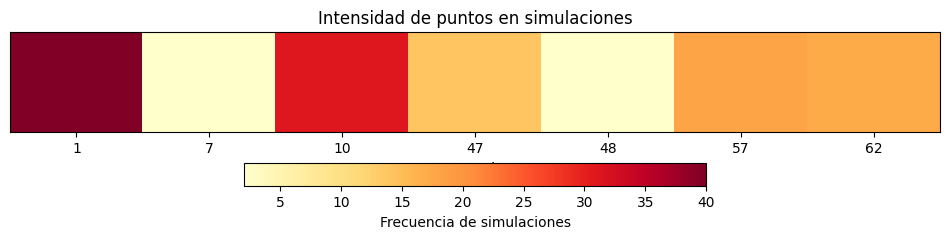
\includegraphics[width=1\linewidth]{launch_stats}
		\caption{Puntos de almuerzo}
		\label{Puntos de almuerzo}
	\end{figure}
	
	\begin{figure}
		\centering
		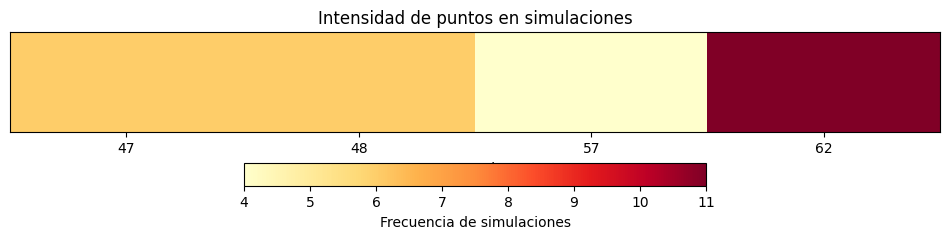
\includegraphics[width=1\linewidth]{reagroup_stats}
		\caption{Puntos de reagrupaci\'on}
		\label{Puntos de reagrupacion}
	\end{figure}

	\begin{figure}
		\centering
		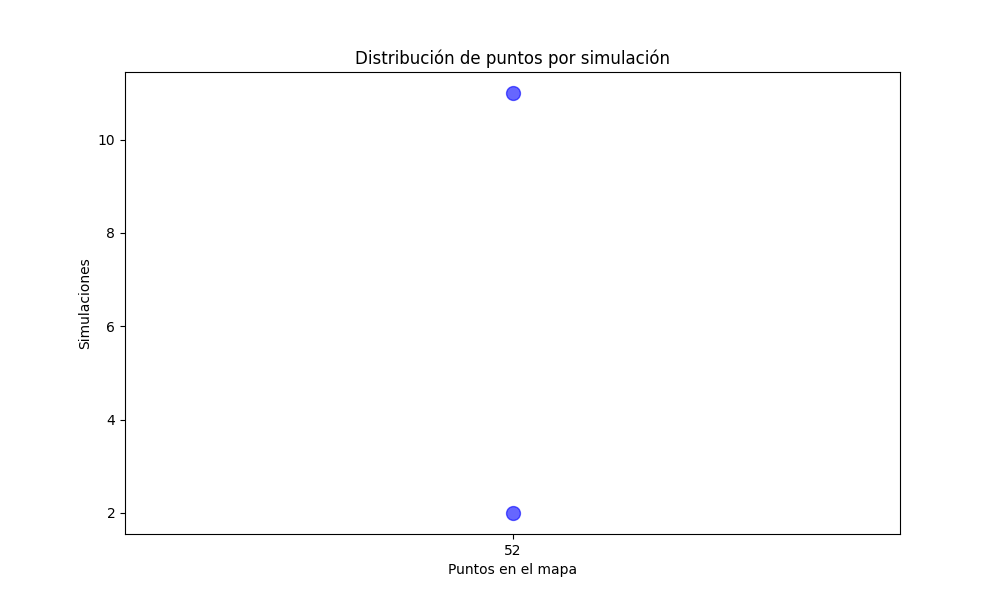
\includegraphics[width=1\linewidth]{camp_stats}
		\caption{Puntos de campamento}
		\label{Puntos de campamento}
	\end{figure}

	
	
	\section{Conclusiones}
	Esta investigación ha demostrado que es posible planificar de manera efectiva una excursión utilizando un modelo de simulación basado en las preferencias individuales de los excursionistas y las características del terreno. El sistema ayuda al guía a identificar los puntos óptimos para descansos, almuerzos y campamentos, garantizando una experiencia más organizada y satisfactoria para el grupo. 
	
	Mediante la recolección de datos previos a la excursión se mejora el disfrute de los campistas. La simulación con agentes BDI y un controlador difuso asegura que la planificación de los puntos clave se adapte a las necesidades del grupo, manteniendo a los excursionistas cohesionados bajo la guía supervisada. Este enfoque ofrece un método eficiente para gestionar excursiones de manera óptima y personalizada.
	
	
	\begin{thebibliography}{9}
		
		\bibitem{Fuzzy} Klir, G. J., \& Yuan, B. (1995). \textit{Fuzzy Sets and Fuzzy Logic: Theory and Applications}. Prentice Hall. Información extraída de las páginas 330-332.
		
	\end{thebibliography}
	
	
\end{document}
